\textbf{Код класса арифметической прогрессии}

\lstinputlisting{paragrafs/Zadachi/7}

В классе присутсвуют функции, которые высчитывают с помощью формул определённый член прогресси, а также сумму прогрессии. 

Во второй части кода пользователь вводит значения, которые передаются в класс и принимаются в качестве аргументов функциями, после чего ответ выводится на экран.

Задачи на арифметическую прогрессию

\begin{figure}[h]
	\centering
	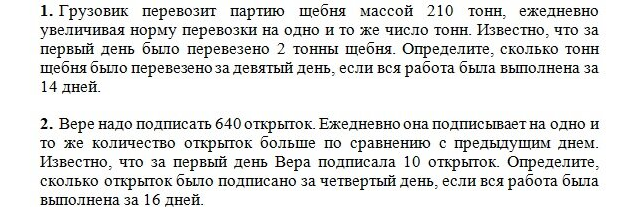
\includegraphics[width=1\linewidth]{VM/ar1.png}
	\end{figure}
	
Шаблон использующий библиотеку со встроенным классом
\\ арифметической прогрессии

\lstinputlisting{paragrafs/Zadachi/10}

\textbf{Задачи, сгенерированные по шаблонам, использующим код
\\арифметической прогрессии.}
	\begin{figure}[h]
		\centering
		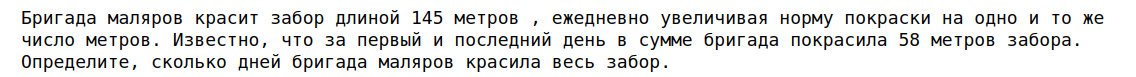
\includegraphics[width=1\linewidth]{VM/121.png}
		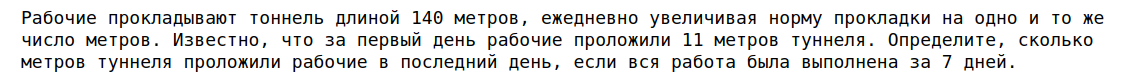
\includegraphics[width=1\linewidth]{VM/221.png}
		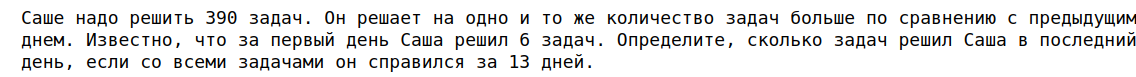
\includegraphics[width=1\linewidth]{VM/321.png}
	\end{figure}


Задачи на геометрическую прогрессию

\begin{figure}[h]
	\centering
	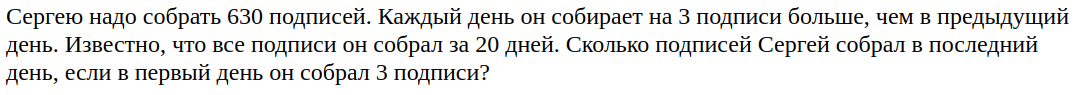
\includegraphics[width=1\linewidth]{VM/ar2.png}
	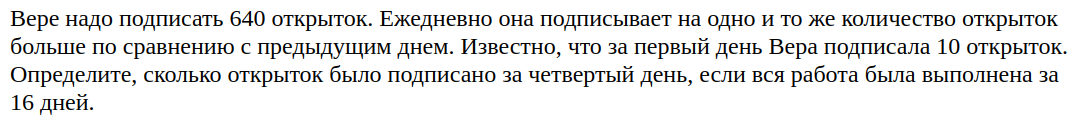
\includegraphics[width=1\linewidth]{VM/ar3.png}
	\end{figure}

\textbf{Код геометрической прогрессии}

\lstinputlisting{paragrafs/Zadachi/8}

Помимо функций вычисления определённого члена прогрессии и её суммы, здесь также пристутсвует функция, вычисляющая сумму бесконечно убывающей прогрессии. Для этого она проверяет, является ли знаменатель прогрессии меньше единицы, и не является ли он меньше нуля, ведь в таком случае прогрессия является знакочередующейся, и следовательно её сумму уже нельзя найти.

 Во второй части пользователь также вводит переменные для прогрессии, и происходит вывод значений на экран.

\textbf{Задачи, сгенерированные по шаблонам, использующим код 
\\геометрической прогрессии.}

	\begin{figure}[h]
		\centering
		
\includegraphics[width=1\linewidth]{VM/421.png}
		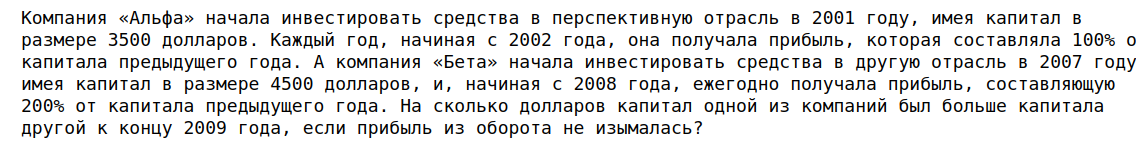
\includegraphics[width=1\linewidth]{VM/521.png}
	\end{figure}
	
